\chapter{Modificación de la Fuente DC anterior}
% ----------------------

\label{C:Sobre la fuente anterior}

\section{Sobre la fuentes de alimentación anterior}
La revisión y adaptación del trabajo previo titulado "Diseño y construcción de una fuente de alimentación DC lineal con control digital de tensión y corriente" llevado a cabo por Eduardo Javier Matijak y Joaquín Pelinski, documentado en su publicación [23], sirve como punto de partida para comprender las mejoras implementadas en la fuente de alimentación DC que se examina en este informe. \cite{Invitamos cordialmente al lector interesado a consultar dicho trabajo para obtener 
una comprensión más completa de los fundamentos sobre los cuales se basa este análisis.}
Este documento se centra en analizar y discutir las modificaciones realizadas en la fuente de alimentación, específicamente la transición de su mayoría analógica a una configuración digital. Entre los principales cambios introducidos se destacan los siguientes aspectos:

\subsection{Circuito Fijador de Referencia para los Transistores}
El circuito fijador de referencia para los transistores ha sido modificado para incorporar la salida de un Convertidor Analógico-Digital (DAC). El DAC es ahora responsable de aplicar niveles de voltaje acorde a los valores determinados por el control digital. Esta modificación permite un ajuste preciso y programable de las referencias de voltaje, eliminando la necesidad de ajustes mecánicos mejorando la precisión y flexibilidad del sistema.
\begin{figure}[H]
    \centering
    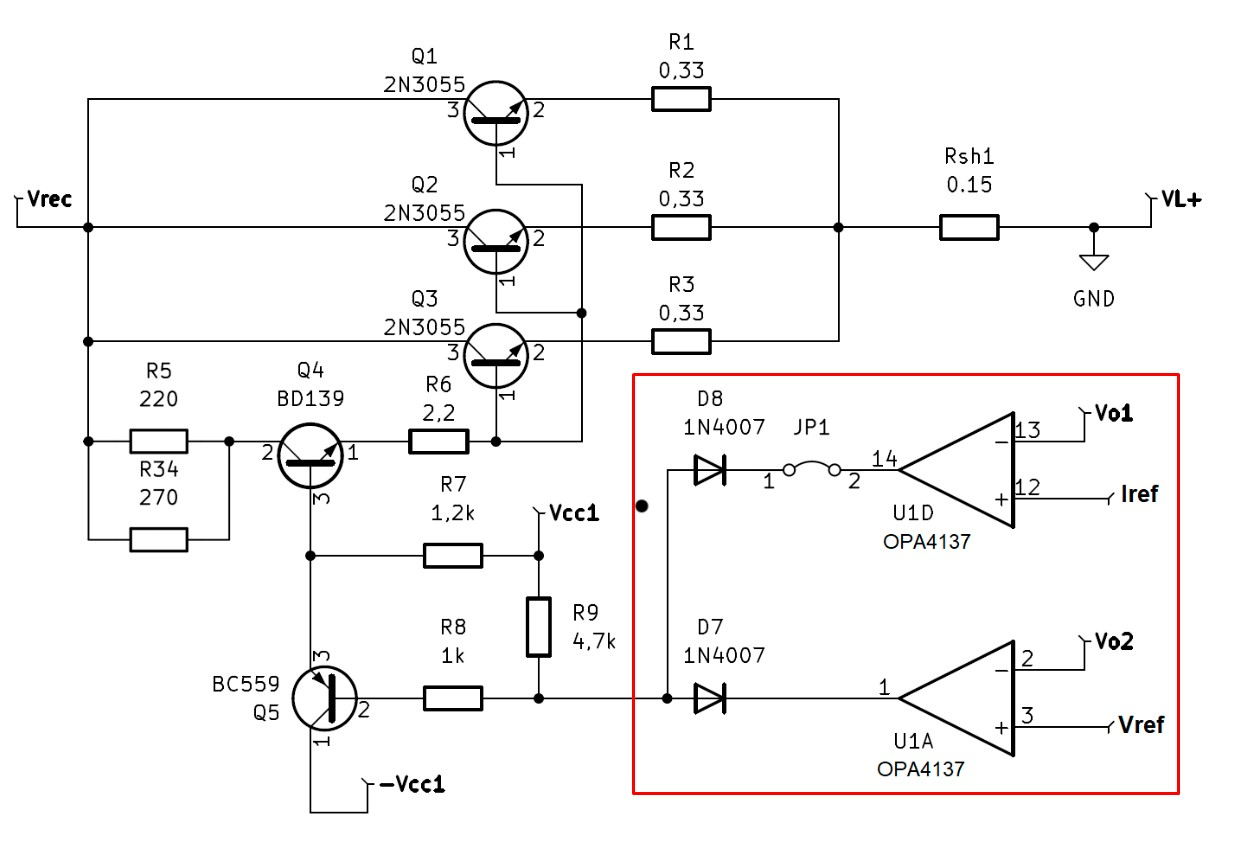
\includegraphics[scale=0.3]{./imagenes/Eliminada1.jpg}
    \caption{Sección de referencia de tensión.}
    \label{F:estructura_archivos}
\end{figure}

\subsection{Modificación de uso de Potenciómetros Digitales MCP4661}
Originalmente, los potenciómetros digitales MCP4661 se utilizaban para establecer una referencia de voltaje que comandaba los transistores, definiendo tanto la tensión como la corriente sobre la carga. Sin embargo, con la incorporación del DAC, esta función ya no es necesaria. En su lugar, los potenciómetros digitales ahora se utilizan para establecer una referencia de tensión destinada a un circuito de protección analógica contra cortocircuitos. Esta reasignación permite una respuesta inmediata para proteger la carga, evitando los retrasos inherentes a los cálculos y actualizaciones de salida necesarios en un sistema de control digital.
\begin{figure}[H]
    \centering
    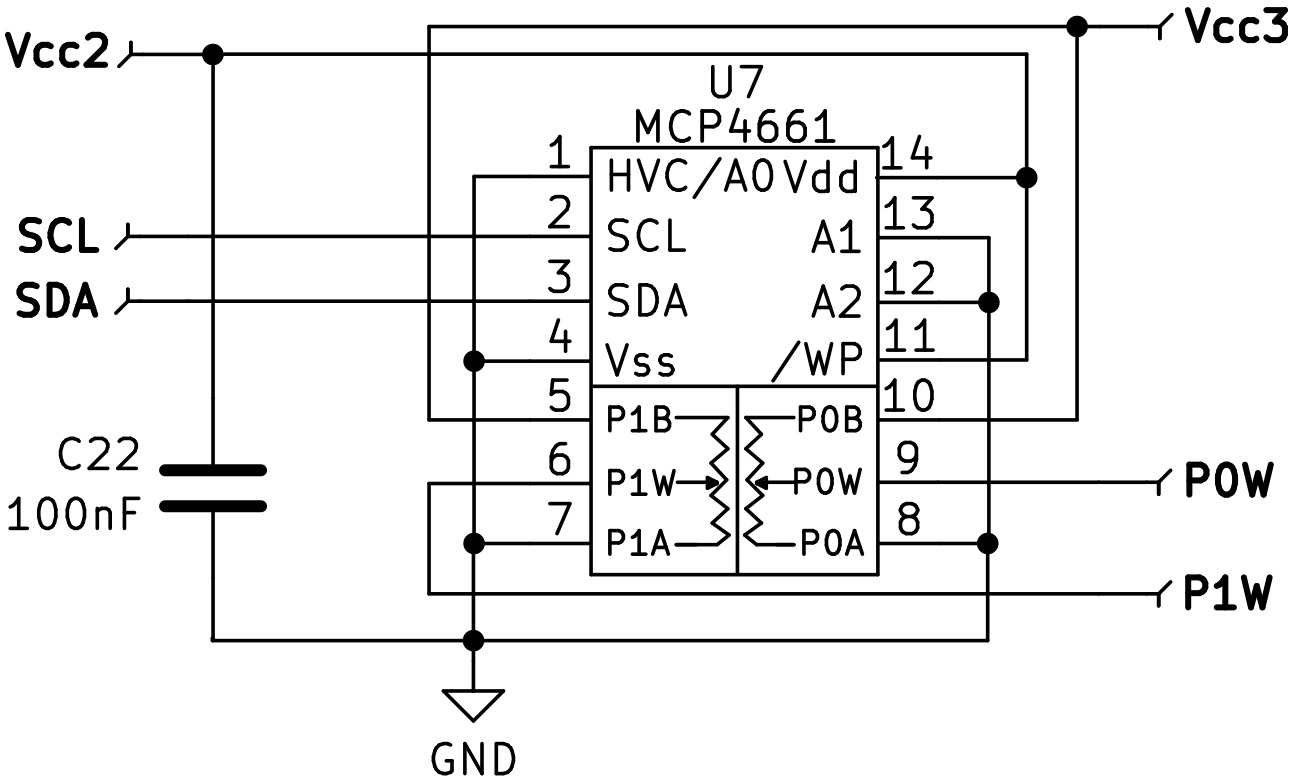
\includegraphics[scale=0.2]{./imagenes/potenciometro_digital.jpg}
    \caption{Potenciómetros digital MCP4661.}
    \label{F:potenciometro_digital}
\end{figure}

\subsection{Eliminación del circuito de medición externo}
Dado que la fuente de alimentación ahora cuenta con una pantalla integrada que muestra en tiempo real los valores de tensión y corriente, el circuito dedicado a la conexión de un voltímetro-amperímetro digital se ha considerado innecesario y, por lo tanto, ha sido eliminado. Esta simplificación reduce la complejidad del diseño y el número de componentes necesarios reduciendo los costos constructivos de la fuente.
\begin{figure}[H]
    \centering
    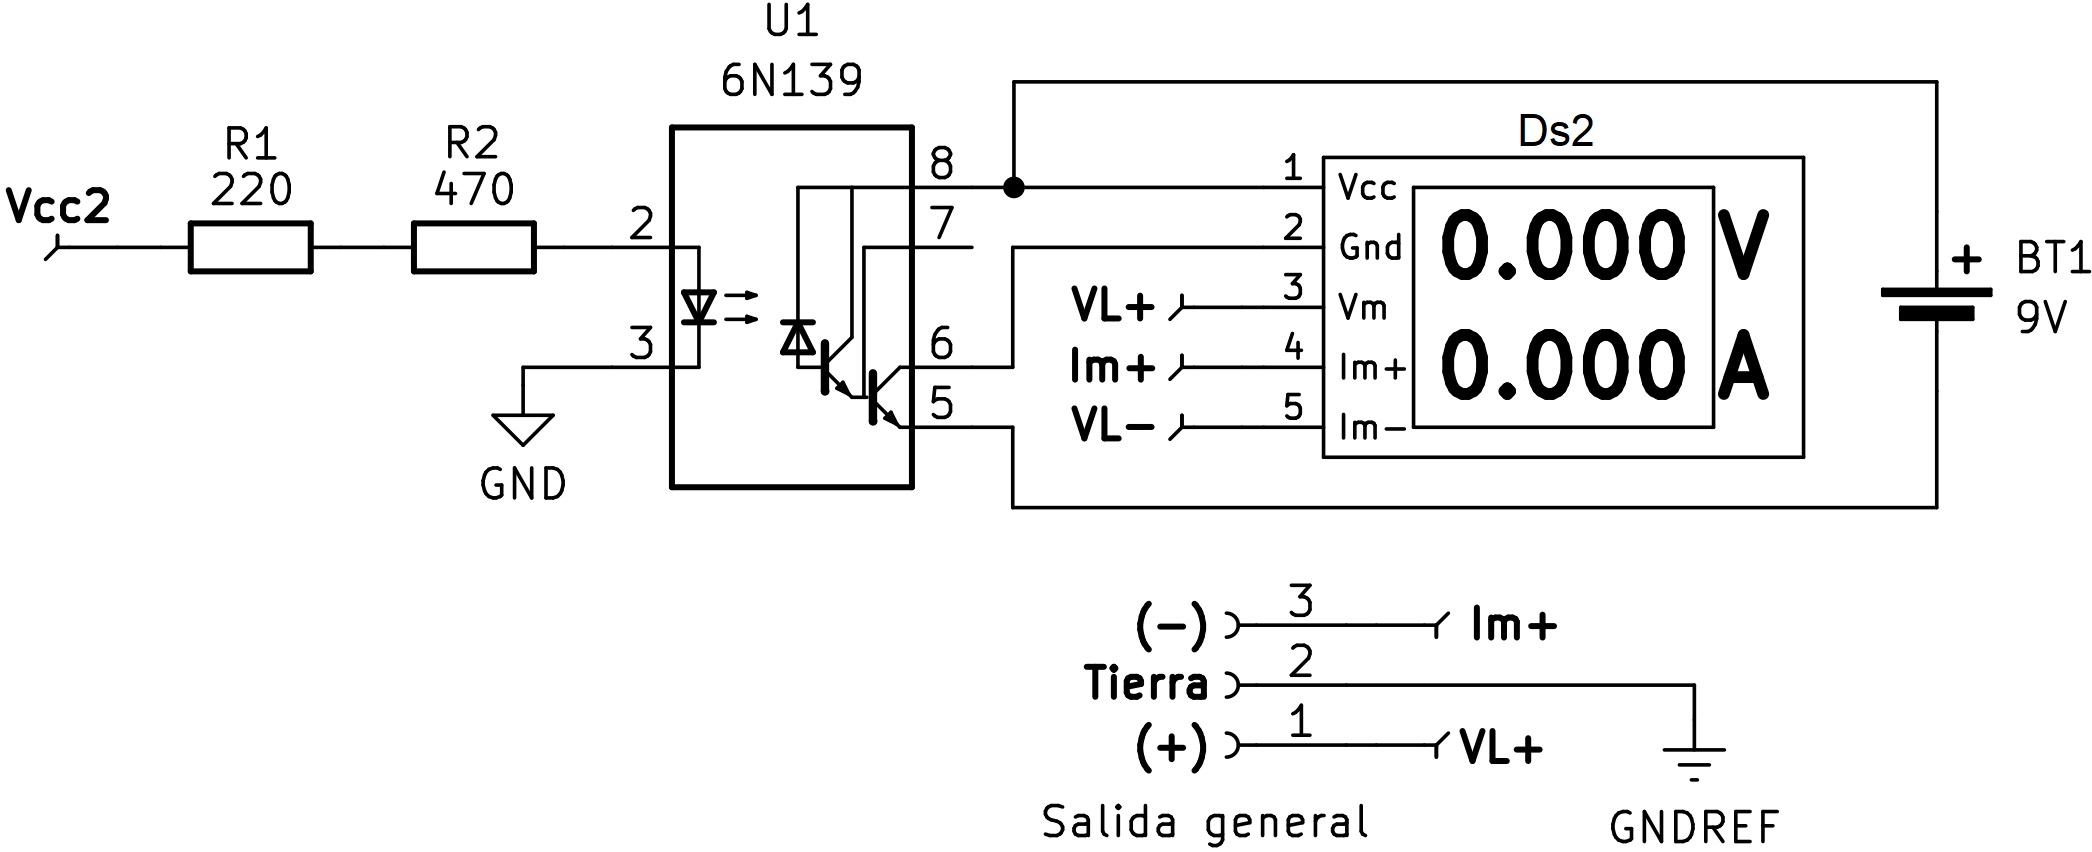
\includegraphics[scale=0.2]{./imagenes/voltimetro_amperimetro.jpg}
    \caption{Conexión voltímetro/amerimetro.}
    \label{F:voltimetro_amperimetro}
\end{figure}

\subsection{Modificación del Circuito de Acople y Desacople de Carga}
Se ha reducido considerablemente el circuito de disparo del optoacoplador, aprovechando las capacidades proporcionadas por el Arduino Nano para establecer un pin en estado alto.
\begin{figure}[H]
    \centering
    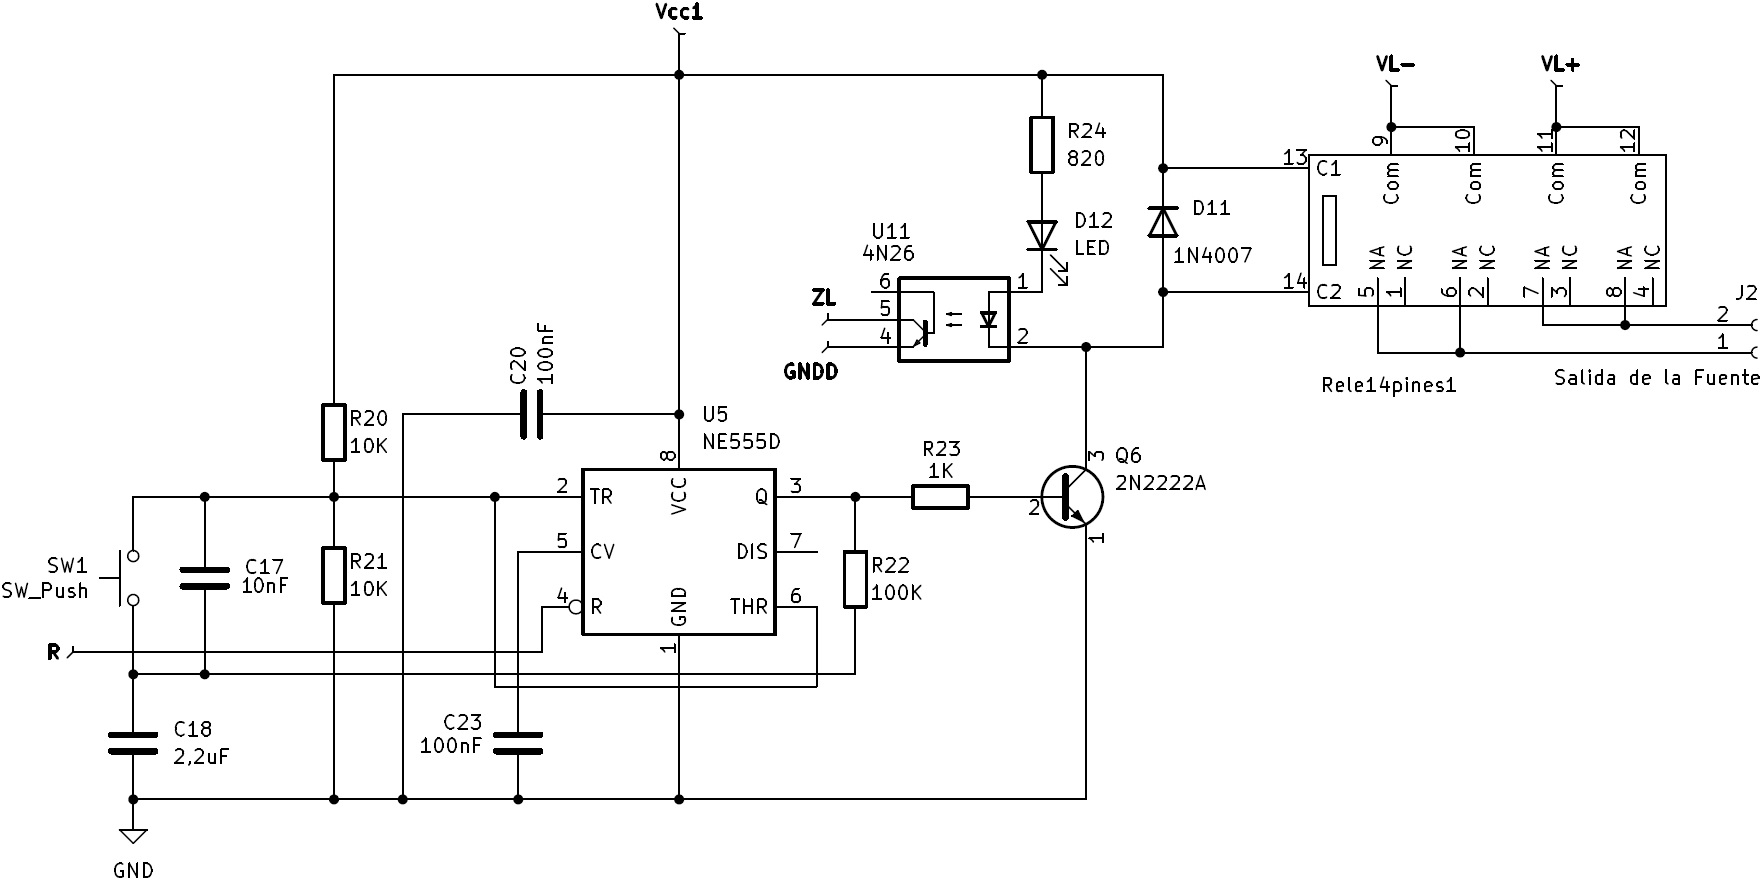
\includegraphics[scale=0.3]{./imagenes/conexion_carga.jpg}
    \caption{Acople y desacople de carga.}
    \label{F:conexion_carga}
\end{figure}

\subsection{Simplificación del Circuito Indicador de Modo de Operación}
La pantalla integrada también cumple la función de indicar el modo de operación, eliminando la necesidad de un circuito adicional dedicado a esta tarea. Esto no solo simplifica el diseño del sistema, sino que también mejora la usabilidad al centralizar toda la información relevante en un solo lugar.
\begin{figure}[H]
    \centering
    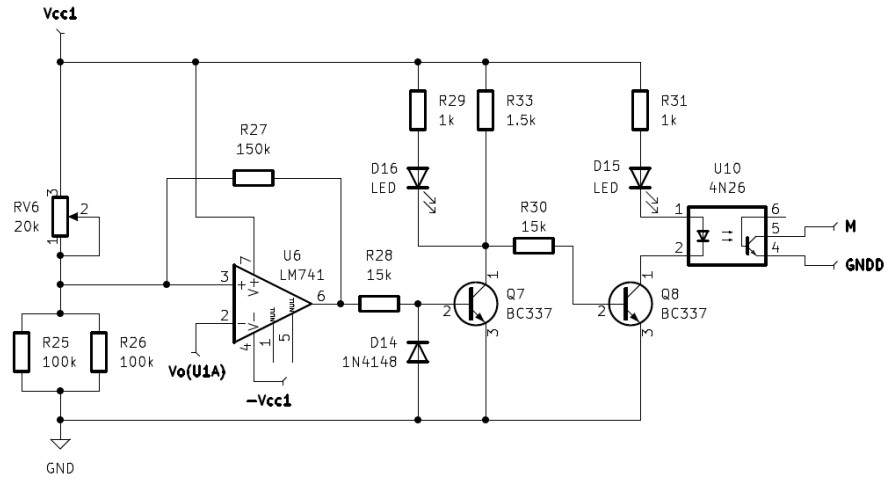
\includegraphics[scale=0.5]{./imagenes/modo_operacion.jpg}
    \caption{Sección de referencia de tensión.}
    \label{F:modo_operacion}
\end{figure}

\subsection{Integración del Circuito con NodeMCU ESP-32S}
Dado que no se requiere una conexión inalámbrica según las especificaciones del circuito, se ha prescindido del microcontrolador ESP con módulo Wi-Fi para visualizar la información en una computadora.
\begin{figure}[H]
    \centering
    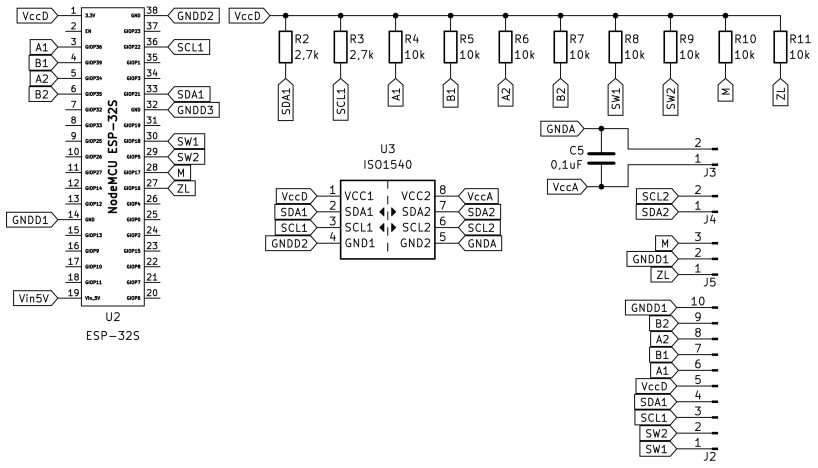
\includegraphics[scale=0.5]{./imagenes/ESP_32S.jpg}
    \caption{Circuito registrador de datos.}
    \label{F:ESP_32S}
\end{figure}

\subsection{Encoders rotativos}
El uso de un teclado numérico hace que este elemento se vuelva totalmente innecesario para estas aplicaciones dado a que el objetivo de la fuente es que sea totalmente digital evitando el ajuste manual de las magnitudes. Sin embargo no habría problema en implementar este elemento en paralelo en caso de un nuevo diseño para seteo de magnitudes, esto debido a una cuestión tradicional ya que la gran mayoría de los usuarios estan acostumbrado a setear manualmente las fuentes de tensión. 
\begin{figure}[H]
    \centering
    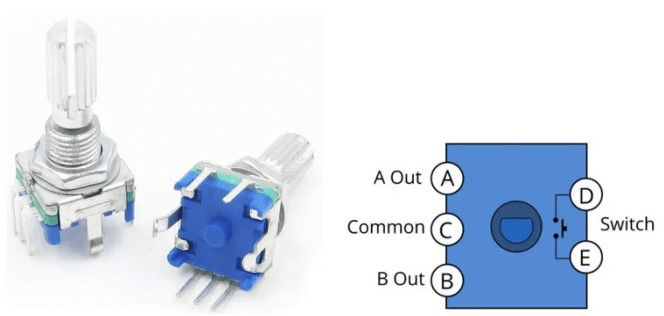
\includegraphics[scale=0.5]{./imagenes/encoder_rotativo.jpg}
    \caption{Encoder rotativos.}
    \label{F:encoder_rotativo}
\end{figure}

Estas modificaciones han permitido no solo modernizar la fuente de alimentación, sino también mejorar su funcionalidad y eficiencia mediante la incorporación de tecnología digital y la simplificación de circuitos redundantes. En las secciones siguientes, se detallarán en profundidad cada uno de estos cambios y su impacto en el rendimiento general del equipo





